Оптимальное распределение ресурсов в аналитических постановках изучается с помощью дизайна механизмов,
предложенных и развитых в работах нобелевского лауреата Л. А. Гурвича  \cite{hurwicz1960optimality}.
Теоретический аппарат механизма широко распространен в экономике и социальных науках, и используется в создании форматов
справедливой и эффективной коллективной деятельности, включающей аукционы, выборы и право благосостояния.

Теория механизмов изучает проблемы доказательной эффективности организации рабочих процессов с учетом
скрытых потребностей исполнителей. Исходя из предположений о рациональности агентов,
механизм определяет правила их поведения для приведения коллективной системы в состояние 
равновесия с оптимальной производственной функцией. Аналитическое описание механизма выполняется через
теорию байесовых игр с неполной информацией.

\textit{Определение:} \textbf{Байесова игра} это набор исходов $(N,O,\Theta)$ таких что:
\begin{itemize}
    \item $\mathbf{N}$ конечное множество агентов $n$;
    \item $O$ множество исходов;
    \item  $\Theta = \Theta_1 \times \Theta_2 \dots \Theta_n $ множество; 
    \item $u = (u_1, \dots, u_N)$, где $u_i: O \times \Theta \rightarrow \mathrm{R}$  функция полезности для игрока $i$.
\end{itemize}

\textit{Определение:} \textbf{Механизм} для байесовой игры это пара $(A,M)$, где: 
\begin{itemize}
    \item $A = A_1 \times \dots \times A_n$ набор действий доступный агенту $i$;
    \item $M: A \rightarrow \Pi(O)$ соединяет действия с распределением возможностей.
\end{itemize}

В заданной игре игроки стремятся к поиску стратегии, ведущей к безусловному преимуществу независимо от
действий прочих игроков. Такие стратегии называются доминантными и являются предметом изучения исследований. 
анализе доминантных стратегий и равновесных состояний, к которым они приводят. 

\textit{Определение:} В заданной байесовой игре, механизм является \textbf{воплощением доминантной стартегии} 
социального выбора функции $C$, если для любого вектора полезности $u$ у игры есть равновесие в 
доминантной стратегии, и для любого равновесия $a^*$ выполняется $M(a^*) = C(u)$.

Теория механизмов используется в постановках с ассиметричной информацией и достаточно большим числом игроков, что, 
как правило, исключает возможность наивного перебора возможных исходов.

\begin{figure}[h]
    \centering
    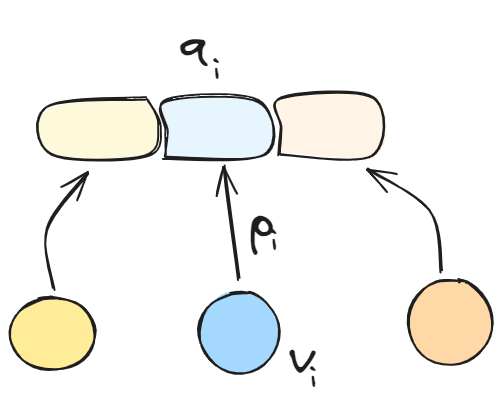
\includegraphics[width=0.5\textwidth]{assets/pedagogic/social/mech.excalidraw.png}
    \caption{Механизм определяет распределение ресурса $\mathbf{x}$ и платежа $\mathbf{p}$ в зависимости от ставок $\mathbf{b}$}
    \label{mech}
\end{figure}

Каждый игрок $i$ имеет четверку $(v_i,b_i,p_i)$, соответствующую:
\begin{itemize}
    \item случайная величина $v_i$ с функцией распределения $F$. Обозначим полученный квантиль распределения $q(v_i) = 1 - F(v_i)$;
    \item ставка на лот $b_i$;
    \item доля полученного ресурса $x_i$;
    \item $p_i$ итоговый платеж.
\end{itemize}

Тогда функция полезности для каждого игрока $i$ при заданном векторе ставок запишется как:
\begin{equation}
    u_i(\mathbf{b};q_i) = v(q_i) \cdot x_i(\mathbf{b})   
\end{equation}

\textit{Определение:} \textbf{Байес-Нэшевым равновесием} называют результат распределения, в котором каждый участник аукциона
максимизирует свою функцию утилитарности $u_i$ как матожидание от квантилей $q_{-i}$:

\begin{equation}
    \max_{\mathbf{q},\mathbf{b}} \mathrm{E}_{\mathbf{q_{-i}}}\left[u_i(\mathbf{b}(\mathbf{q});q_i)\right] 
\end{equation}

При изучении свойств механизмов разделяется фактически (от \textit{англ.} ex-post) распределенное число ресурсов $\tilde{x}_i(\mathbf{q}) = x_i(\mathbf{b}(\mathbf{q}))$
на игрока $i$ и в среднем ожидаемое (от \textit{англ.} interim) $\hat{x}_i(q_i) = \mathrm{E}_\mathbf{q} \left[\tilde{x_i}(\mathbf{q})|q_i\right]$.
Специфика связана с тем, что среднее ожидаемое доступно к расчету прочими игроками и потому может учитываться при принятии решений \cite{bulow1989simple}.

\textit{Лемма:} Набор имеет Байес-Нэшево равновесие при условии:
 \begin{itemize}
    \item $\hat{x_i}(q_i)$ монотонно убывает по $q_i$;
    \item $\hat{p}_i(q_i) = \mathbb{E}_{\mathbf{q}}\left[p_i(\mathbf{b}(\mathbf{q}))|q_i\right] = v(q_i) \cdot \hat{x}_i(q_i) + \int_{q_i}^1 \hat{x}_i \cdot v'(z) dz$, где $\hat{p}_i$ соответствует ожидаемому платежу игрока.
\end{itemize}
Заданные условия достаточны для достижения уникального равновесия $\mathbf{b}$. Доказательство приведено в \cite{myerson1981optimal}.
Одним из примером механизма являются рейтинг-системы, широко распространенные в спортивных интеллектуальных соревнованиях.

\textit{Определение:} \textbf{Рейтинг-система} --- модель, ранжирующая $n$ участников в единый линейный порядок $i_1 \succ i_2 \succ \dots i_n$
по данным сравнений небольших подмножеств этих игроков.
 
Статистический подход к введению рейтинг-моделей заключается \cite{bradley1952rank} 
в введении вероятности победы в ходе отбора объекта $i$ над объектов  $j$:
\begin{equation}
    p(x_i \succ x_j) = \zeta(x_i,x_j),
\end{equation}
где функция $\zeta$, принимает на вход скалярные потенциалы $x_i$ и $x_j$, соответствующие силе объектов.

Вид функции сравнения $\zeta$, в общем случае, не определен и выбирается на основании статистических исследований.
В работе \cite{elo1967proposed} Арпад Эло на основании данных шахматной федерации США предложил
для стратегических игр использование логистической функции:
\begin{equation}
    p(x_i \succ x_j) = \frac{1}{1 + exp(-\frac{x_i- x_j}{\sigma})},
    \label{elo_prob}
\end{equation}
где дисперсия $\sigma$ фиксирована для всех игроков. Отличительной чертой такой модели является
гарантия победы игрока с значимо большим навыком $x_i- x_j \gg \sigma$.

Отметим, что система Эло также задает правило обновления рейтинга обеспечивающих эволюций системы рейтинга во времени. 
Обновление рейтинга $R$ игрока выполняется по исходу игры $S$ в соревновании согласно правилу:
\begin{equation}
    R' = R + \sigma (S-p),
\end{equation}
где $R'$ --- новый рейтинг игрока, $p$ --- вероятность победы в матче согласно \ref{elo_prob}.
Новые очки рейтинга поступают в систему с появлением новых участников. В шахматной практике игроки начинают
с рейтингом 1600.


